\documentclass[a4paper,11pt, oneside]{article}  % document class
\usepackage{geometry}
\geometry{
  inner=20mm,
  outer=20mm,
  top=27mm,
  bottom=25mm %
%  heightrounded,
%  marginparwidth=50pt,
%  marginparsep=17pt,
%  headsep=20pt
}
\usepackage[english]{babel}
\usepackage{hyperref}
%pacchetto
\usepackage{import, multicol,lipsum}  % package
\setlength{\columnsep}{1cm}

\usepackage[utf8]{inputenc} % accenti facili
\usepackage[T1]{fontenc}
\usepackage{subcaption}
\usepackage{pifont}
\usepackage{url}
\hypersetup{
	colorlinks=true,
	linkcolor=blue,
	filecolor=magenta,      
	urlcolor=blue
}
\usepackage{graphicx, color, blindtext}
\usepackage{textcomp, makeidx, times}
\usepackage{amsthm, amsmath, amssymb, amsfonts, mathtools} % math
\usepackage[mathscr]{eucal}		
\usepackage[nottoc]{tocbibind} 
\usepackage{pgfplots, parskip}
\usepackage{afterpage, ifthen}
\usepackage{enumitem}
\pgfplotsset{compat=newest}
\usepackage{graphicx} % immagini
\usepackage{wrapfig}
%\graphicspath{ {image/} } % path cartella delle immagini
\usepackage{tikz} %graph
\usetikzlibrary{arrows,automata}
\usetikzlibrary{automata,arrows,positioning,calc,matrix}
\usepackage[linesnumbered,ruled,vlined]{algorithm2e}
\usepackage{booktabs}
\usepackage{colortbl}
\usepackage{siunitx}
\usepackage{tabularx, tabu}
\usepackage{relsize}
\usepackage{makecell, caption, chngcntr}
\usepackage{bbm}
\usepackage{diffcoeff}
\RequirePackage{fix-cm}


%
%____________________________________________________________________________________________________________________________
%____________________________________________________________________________________________________________________________
%____________________________________________________________________________________________________________________________
%____________________________________________________________________________________________________________________________
% INIZIO
\begin{document}

\setcounter{secnumdepth}{2}
\pagestyle{plain} % stile pagina (header, numerazioni)

\centerline {
\includegraphics[width=2cm]{logo.jpg}}
\begin{center}
	Università degli Studi di Torino - M.Sc.  in Stochastic and Data Science - A.Y.  2021/2022 \\
	\Large { Final project of Statistical Machine Learning (MAT0043)}
	\line(1,0){450}\\ 
	\vspace{0.4cm} 
	{ \huge \textbf{Gene selection for cancer type classification} }
	\vspace{0.1cm}
	\line(1,0){450} \\
\end{center}

%____________________________________________________________________________________________________________________________

The purpose of our project is to work on a high-dimensional genomics data and find a relatively small number of genes to predict the cancer type of a given tumorous cells. This is known as Genes Selection for Cancer Classification and it is in line with many up-to-date problems of applied medicine. \\
Our dataset contained $1.032$ cancerous cells and their knock-out probabilities, i.e. the probabilities of stopping the growth of tumor by inhibiting one of the $\sim 17.000$ genes. Each cell line was characterized by one of 10 possible cancer labels: Eye, Gastrointestinal, Gynecologic, Musculoskeletal, Neurological, Breast, Head-Neck, Hematologic, Genitourinary and, finally, Lung. We explored in details three Features Selection algorithms: Random Forests (RF) combined with Feature Importance, Lasso-SVM and Neural Networks (NN) combined with Olden Importance.  We studied two binary classification problems (Blood-cancer vs. All, Lung-cancer vs. All) and the multiclass problem. Besides lung models, we achieved satisfying classification accuracies and we were able to select about $100$-$200$ genes from the initial $\sim 17.000$ ones. Models fitted on such genes obtained classification accuracies ranging from $67\%$ to $98\%$. \\
Therefore, it seems that classifying cancer type from an extremely small set of genes depends on the cancer type itself. These methodologies worked incredibly well on Blood cancer, as  we reached almost $100\%$ accuracy with the reduced classifier,  while failed miserably on Lung cancer.  


\section{Introduction}
Cancer is a complex disease characterized by the uncontrolled growth of abnormal cells anywhere in the body. These abnormal cells are extremely invasive and we usually identify them with the name of their original tissue (for instance, breast cancer, lung cancer,  brain cancer, etc.).  In recent years, medicine has made a great step forward in finding new and efficient therapies for different diseases and cancer is one of them.  In particular,  thanks to numerous advances in technology,  collecting huge amount of data is no longer an issue, so that one can exploit such information to define personalized treatments for patients. In this regards, the DepMap project\footnote{DepMap Portal: \url{https://depmap.org/portal/} } and,  in particular,  the Achilles project\footnote{Achilles Project: \url{https://depmap.org/portal/achilles/} } aim to use genome-wide screens to collect data regarding mutations of cancerous cells,  identify essential genes and report vulnerabilities across hundreds of human cancers.  \\
 
Many researches are currently using DepMap datasets to identify relatively small sets of genes which are responsible of cancers growth\footnote{Background material: \url{https://depmap.org/portal/publications/}}. This procedure is often driven by medical knowledge,  which we do not possess,  together with some rough measures of importance.  Being Maths student,  we instead base our research on statistical models and on the hypothesis that, if a given classifier is able to distinguish different types of cancer, then the most relevant genes are the most important features for that classifier (the meaning of "important features" will be clarified later).  Of course,  selecting few truly significant genes has outstanding implications in the medical field: building faster diagnosis tools and synthesizing less toxic drugs are only two examples. 


\section{Dataset}
We used two public datasets from the DepMap Public 21Q3 database,  released on August 2021\footnote{Download dataset from DepMap:  \url{https://depmap.org/portal/download/}}:
\begin{itemize}
	\item[D1] \textit{CRISPR\_gene\_dependency.csv},  which contains $1.032$ cancer cell lines characterised by $17.393$ gene scoring results
	\item[D2] \textit{sample\_info.csv}, which contains cell lines information,  such as primary disease and sample collection site
\end{itemize}
Data were collected from real patients and successively processed,  so that element $(i, j)$ of this $(1.032 \times 17.393)$-data frame is the probability that knocking out gene $j$ has a real depletion effect on the $i$-th cell.
Before proceeding with our analysis, we removed missing values, which affected only 10 rows coming from different tumours, and we looked for weird observation. In particular, we found $2$ "Non-Cancerous" and $6$ "Engineered" cells. The first can be reasonably discarded, whereas the latter requires a little care. Engineered cells are synthetically modified samples in lab and, here, they are manly associated to the Eye sample collection site. We decided to keep them and associate them to the cancer corresponding to their site. \\

\begin{wrapfigure}{r}{0.65\textwidth}
	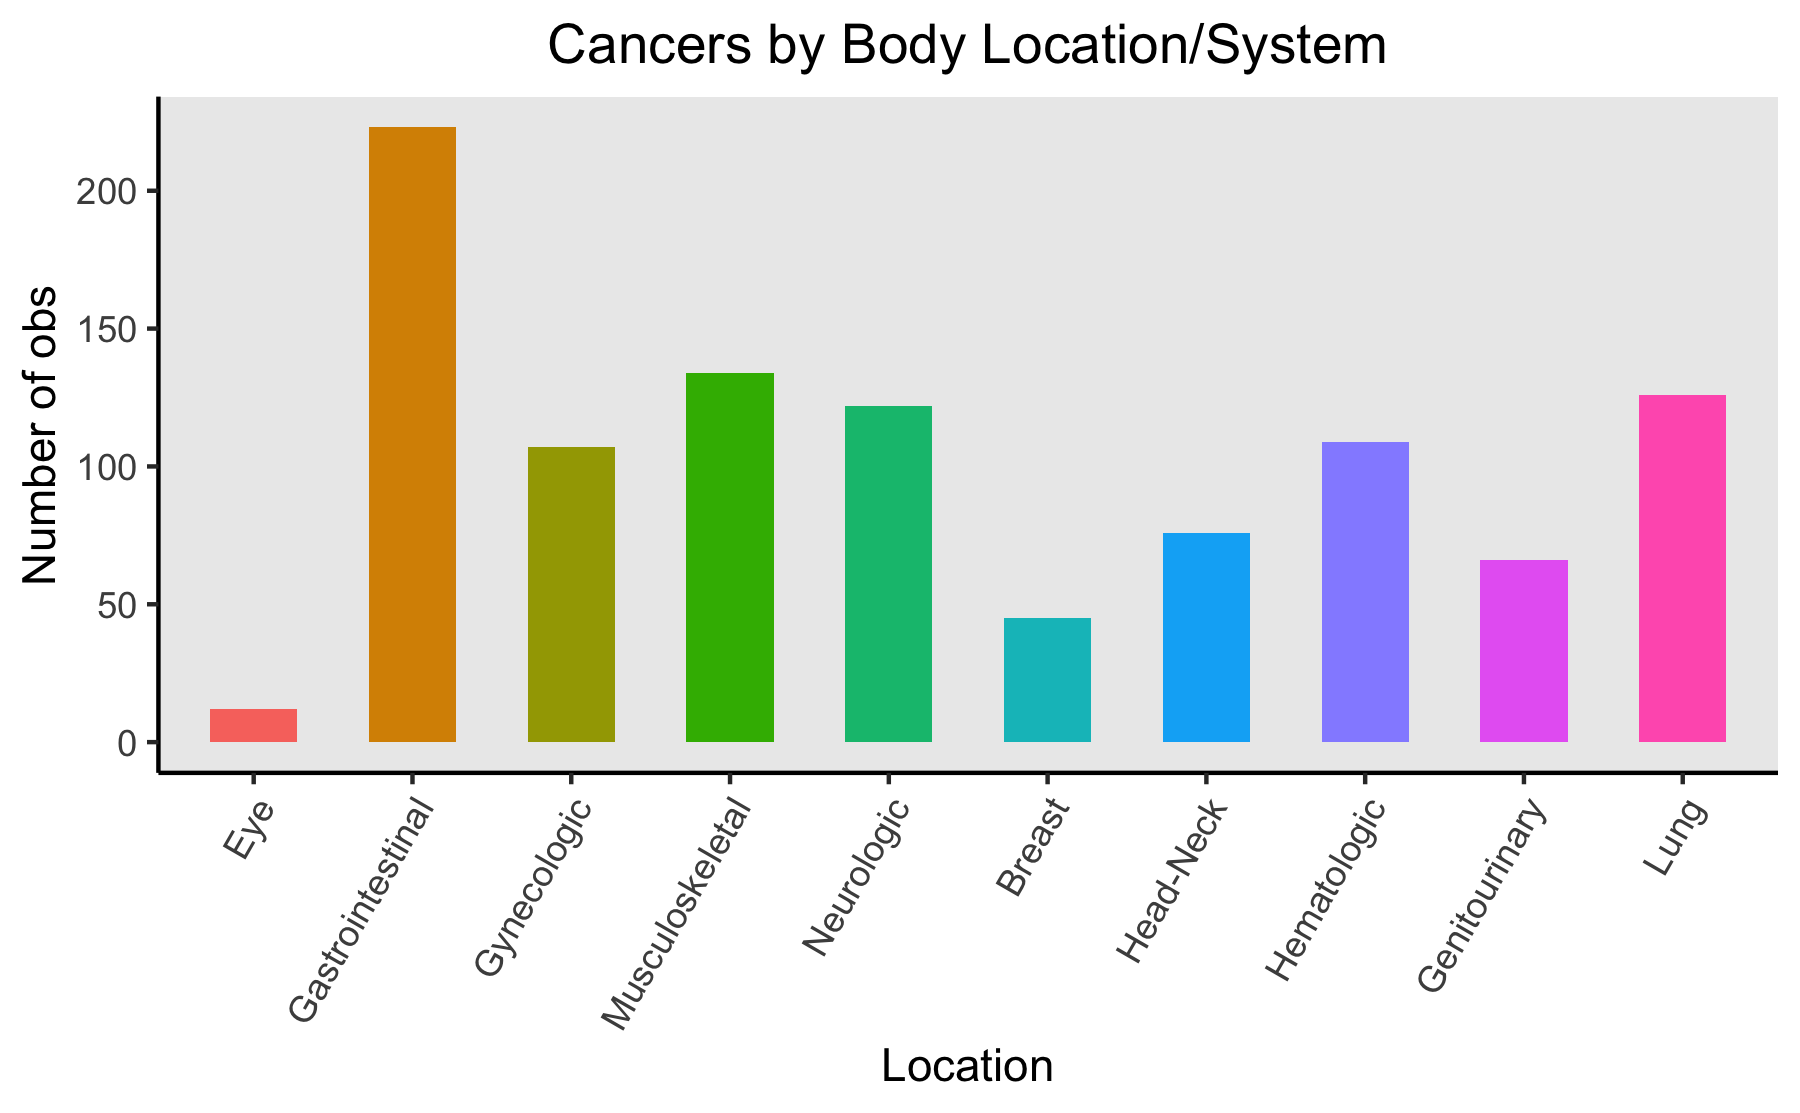
\includegraphics[width=0.65\textwidth]{plot1.png}
	\captionof{figure}{Cancer classes}\label{fig1}
\end{wrapfigure}

We  grouped the various cancer types in 10 classes according to common medical knowledge\footnote{Cancer types grouped by body location: \url{https://www.cancer.gov/types/by-body-location}} and we obtained classes as reported in Figure \ref{fig1}.  "Eye" is the smallest one as there are only $16$ observations, $5$ of which labelled as "Enginereed". On the other hand, "Gastrointestinal" is the largest group and it comprehends $7$ types of cancer,  making this group quite heterogeneous.
We decide to investigate two binary classification problems,  Blood vs Rest and Lung vs Rest, and the multiclass problem. We chose Lung because of the nature of such a class: it is the most numerous group composed only by Lung cancer samples. The choice of Blood was instead driven by some underlying biological knowledge. In fact,  Blood cancer is quite different from other tumours because
\begin{itemize}
	\item blood is in the whole body
	\item Leukemia, Lymphom and Myeloma are the main kinds of cancer but they all affect white blood cells
	\item not all blood cancers require a treatment, just periodical monitoring
\end{itemize} 


\section{Methods}
This section deals with a brief explanation of the algorithms we used.  Each procedure is characterized by three steps:
\begin{enumerate}
\item fit the model using all the features
\item identify the most important ones based on some measure of importance
\item use these genes to fit a reduced version of the classifier and see how it performs
\end{enumerate}
Clearly,  each procedure involves fitting a model twice,  the all-features version and the reduced version.  Since the latter depends on the former through the selection of the important features it uses,  we were forced to split the dataset into two smaller chunks and to use the first one for point 1 and the second one for point 3.  This is crucial as it ensures the independence of the two models and removes any sort of correlation. 

\subsection{Random Forest}
We started by fitting Random Forest (RF) models as they frequently performs well on imbalanced data and correlated high-dimensional data.  Once the model had been fitted,  we used Variable Importance of RFs to identify the most important features. This measure is calculated in three steps.  First, prediction accuracy are measured on the out-of-bag samples. Then the values of the variable are randomly shuffled, keeping all other variables the same. Finally, the decrease in prediction accuracy on the shuffled data is measured and the mean decrease in accuracy across all trees is reported. Intuitively, the random shuffling means that, on average, the shuffled variable has no predictive power. This importance is a measure of by how much removing a variable decreases accuracy, and vice versa. \\
We used this Variable Importance measure to select the most important feature in two different ways:
%\begin{wrapfigure}{l}{0.3\textwidth}
%	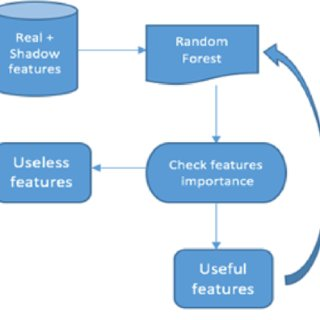
\includegraphics[width=0.3\textwidth]{Boruta-algo.jpg}\label{fig2}
%\end{wrapfigure}

\begin{itemize}
	\item \textit{Cross-validation}. We perfomed a 5-fold cross-validation on the model, selected the top most important features of each model and finally averaged.
	\item \textit{Boruta algorithm}\footnote{Boruta: \url{https://www.researchgate.net/publication/220443685_Boruta_-_A_System_for_Feature_Selection}}: Boruta repeatedly measures feature importance then carries out statistical tests to screen out the features which are irrelevant. 
\end{itemize} 


\subsection{SVM-Lasso}
Support vector machines (SVM) are based on the idea of finding a hyperplane that best separate classes. Here, we combine this method with the classical Lasso penalty,  so that the objective function to be minimized is:
\begin{equation*}
	\dfrac{1}{n} \sum_{i=1}^n hingeLoss(y_i(x_i w + t)) + \lambda \sum_{j=1}^p |w_j|  \qquad	\text{where} \qquad  hingeLoss(z) = max\{0, 1-z\}
\end{equation*}
where the parameter $\lambda$ is chosen via cross-validation.  We then obtain the sparsity in predictors: some $w_i$ are shrunken all the way to zero while the ones that are not will be used to identify the important features. 

\subsection{Neural Networks}
Neural Networks (NN) are efficient models to capture non-linear relationship between the predictors and the target variables.  In this context we trained NN with two hidden layers of width 400 and 300 respectively using  the \textit{ReLU} function as activation  for the hidden layer and the \textit{sigmoid} in the binary classification problem and the \textit{softmax} in the multiclass one for the output layer.  Furthermore,  being the binary classification problems a little unbalanced,  a part from the usual \textit{Cross Entropy} loss function we also used the \textit{Focal Loss}, which is defined as $$ FL(z) = \alpha \cdot (1 - z)^{\gamma} \log{z} \text{,  \hspace{3pt} with }z \in [0,1]  \text{ and } \alpha,  \gamma \geq 0$$ in order to focus learning on hard negative examples.  Note that \textit{Focal Loss} can be extended and used in mutliclass classification tasks as well\footnote{Focal Loss: \url{https://arxiv.org/pdf/1708.02002.pdf}}.  Once this NNs were fitted,  we ranked the variable according to the Olden Importance measure\footnote{Olden Importance: \url{https://depts.washington.edu/oldenlab/wordpress/wp-content/uploads/2013/03/EcologicalModelling_2004.pdf}}, selected the first 120 and used them to construct a reduced version of the classifier.



\section{Results}
\subsection{Binary classifications}

%PCA
Before starting our Binary classifications on Blood and Lung cancer, we ran a Principal Component Analysis to gain some valuable insights. We noticed a surprising result: even if observations formed a cloud of points, Blood cancer cells were mainly concentrated in just one part of the 3-dimensional plot. The same did not happen for Lung cancer observations.

%RF
We then moved to RF classifiers.  %scrivi la tua parte

%SVM


%NN
As for the implementation of NNs,  we firstly fit a single 




\begin{table}[ht]
\caption{Average recall of the models fitted with all the features}
\centering
\begin{tabular}{c c c c}
\hline\hline
Task & RF & SVM-Lasso & NN \\ [0.5ex] % inserts table %heading
\hline
Blood & 50 & 837 & 970 \\
Lung &47 & 877 & 230 \\
Multiclass & 45 & 300 & 556 \\ [1ex]
\hline
\end{tabular}
\label{table:big_models}
\end{table}

\begin{table}[ht]
\caption{Selected variables}
\centering
\begin{tabular}{c c c c c}
\hline\hline
Task & RF & Boruta & SVM-Lasso & NN \\ [0.5ex] % inserts table %heading
\hline
Blood & 50 &837 & 23 & 970 \\
Lung &47 & 877 & 44 & 230 \\
Multiclass & 45 &  44 & 300 & 556 \\ [1ex]
\hline
\end{tabular}
\label{table:selected variables}
\end{table}

\begin{table}[ht]
\caption{Average recall of reduced models}
\centering
\begin{tabular}{c c c c}
\hline\hline
Task & RF & SVM-Lasso & NN \\ [0.5ex] % inserts table %heading
\hline
Blood & 50 &837 & 970 \\
Multiclass & 45 &  44 & 300 \\ [1ex]
\hline
\end{tabular}
\label{table:reduced_models}
\end{table}





\subsection{Multiclass classification}
When working with the multiclass problem we decided to remove the group "Eye" because it was a small heterogeneous group that even after tuning for RF and NN held the worst accuracy scores. "Eye" was a cluster of different types of cancer: this didn't create problems when we were using a One vs All aproach but with multiclass the effects of doing the cluster ourselves was mor evident.  
So after removing the group "Eye", we did the same as before and split the dataset in two.

\subsubsection{Random Forests}
We considered two different random forests, the first with the same parametes as the one used in Blood vs All random forest. Looking at the confusion matrix we can see hat most of the missclassification errors are data points classified as Gastrointestinal. Gastrointestinal was the biggest cluster we consider with a lot of different cancers so the genes( i.e. the features) important can be different within the cluster. To limit the weight of Gastrointestinal we decided to tune by hand the class weights. In this way we solve two problems: we reduced the importance of the group Gastrointestinal and we achieved at least one correct classification in each class. At this point we used cross validation to select five models and we extracted the most important features by looking at their relative importance in every model subjected to their presence in every model. We set a threshold to obtain  $(\sim   1700)$ features and with this we created a reduced model that we fitted using the validation set we had created at the beginning.
\subsubsection{SVM-Lasso}

\subsubsection{Neural Networks}
We first fitted a toy NN with only one hidden layer to see how the net worked.
We then fitted three different NN: the first increasing by one the number of hidden layers, the second changing the loss function with the Focal loss and the third using again the Focal loss, but changing the alpha parameter w.r.t. the class percentage in the set.
The three models held similar result with the second one being slightly more accurate. Once this NNs were fitted, we ranked the variable according to the Olden Importance measure, selected the first 1700 and used them to construct a reduced version of the classifier on the validation set.
The increment in the number of feature used for fitting the reduced model w.r.t. the binary NN model was beacuse we are now trying to separate nine different classes so we need much more information than before.

\section{Overall Results}
We approached the multiclass problem using three different techniques: RF, NN, SVM-Lasso and all three methods gave us good results. We can't say the same for the reduced models: while NN maintain an overall good performance using the same models, the RF need to be retuned to reach a similar performance. 


\section{Conclusion and future works}


%\end{multicols}
\end{document}
